\documentclass[border=12pt]{standalone}
% shared preamble for all schematics/diagrams
\usepackage[siunitx, RPvoltages, european resistors]{circuitikz}
\usepackage{tikz}
\usetikzlibrary{arrows.meta,positioning,calc,shapes.geometric,fit,backgrounds,decorations.pathreplacing}
\usepackage[scaled=0.92]{helvet}
\renewcommand{\familydefault}{\sfdefault}
\usepackage{xcolor}
\usepackage{amsmath}
\usepackage{ifthen}
\definecolor{ink}{HTML}{1F2328}
\definecolor{muted}{HTML}{6B6A66}
\definecolor{c1}{HTML}{2A78D6}
\definecolor{c2}{HTML}{EB6834}
\definecolor{c3}{HTML}{1BAF7A}
\definecolor{c4}{HTML}{6250D6}
\definecolor{fill1}{HTML}{EAF2FC}
\definecolor{fill2}{HTML}{FDEEE7}
\definecolor{fill3}{HTML}{E6F6EF}
\definecolor{fill4}{HTML}{EFEDFB}
\definecolor{hv}{HTML}{C62828}
\ctikzset{bipoles/thickness=1.2, monopoles/ground/thickness=1.2}
\tikzset{every picture/.style={line width=0.7pt, color=ink}}

\begin{document}
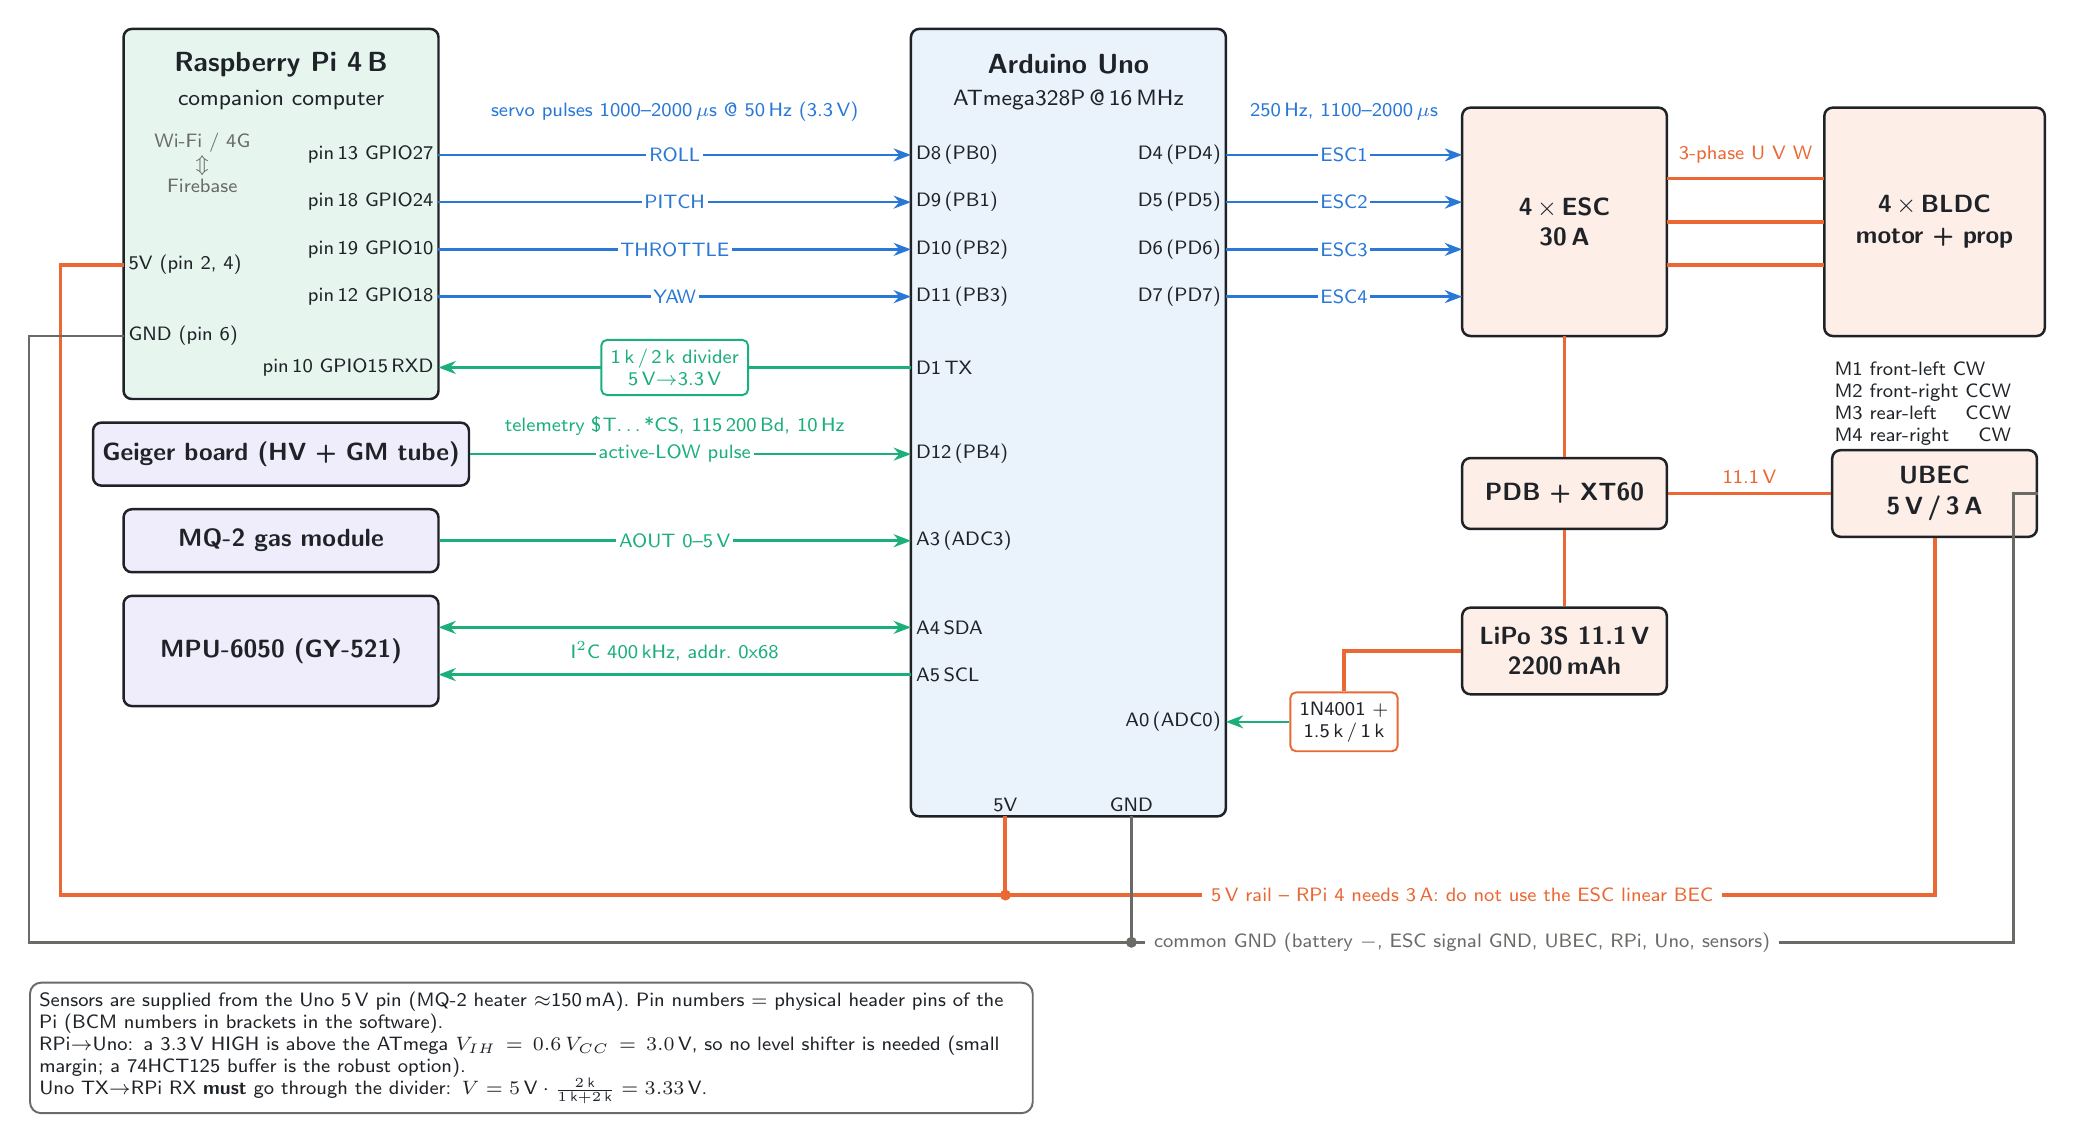
\begin{tikzpicture}[
  blk/.style={draw, rounded corners=3pt, line width=0.9pt, fill=#1, align=center, font=\bfseries\small},
  pin/.style={font=\scriptsize, inner sep=1.5pt},
  lab/.style={font=\scriptsize, inner sep=1pt, fill=white},
  sig/.style={line width=0.9pt, c1},
  pwr/.style={line width=1.4pt, c2},
  gnd/.style={line width=1.0pt, muted},
  dat/.style={line width=0.9pt, c3},
  arr/.style={-{Stealth[length=2.2mm]}},
  dot/.style={circle, fill, inner sep=1.4pt}]

% ================= Arduino Uno =================
\draw[rounded corners=3pt, line width=0.9pt, fill=fill1] (-2,-5.4) rectangle (2,4.6);
\node[font=\bfseries] at (0,4.15) {Arduino Uno};
\node[font=\footnotesize] at (0,3.7) {ATmega328P\,@\,16\,MHz};
\foreach \y/\t in {3.0/D8\,(PB0), 2.4/D9\,(PB1), 1.8/D10\,(PB2), 1.2/D11\,(PB3), 0.3/D1\,TX, -0.8/D12\,(PB4), -1.9/A3\,(ADC3), -3.0/A4\,SDA, -3.6/A5\,SCL}
  \node[pin, anchor=west] at (-2,\y) {\t};
\foreach \y/\t in {3.0/D4\,(PD4), 2.4/D5\,(PD5), 1.8/D6\,(PD6), 1.2/D7\,(PD7), -4.2/A0\,(ADC0)}
  \node[pin, anchor=east] at (2,\y) {\t};
\node[pin, anchor=south] at (-0.8,-5.4) {5V};
\node[pin, anchor=south] at (0.8,-5.4) {GND};

% ================= Raspberry Pi =================
\draw[rounded corners=3pt, line width=0.9pt, fill=fill3] (-12,-0.1) rectangle (-8,4.6);
\node[font=\bfseries] at (-10,4.15) {Raspberry Pi 4\,B};
\node[font=\footnotesize] at (-10,3.7) {companion computer};
\foreach \y/\t in {3.0/pin\,13 GPIO27, 2.4/pin\,18 GPIO24, 1.8/pin\,19 GPIO10, 1.2/pin\,12 GPIO18, 0.3/pin\,10 GPIO15\,RXD}
  \node[pin, anchor=east] at (-8,\y) {\t};
\node[pin, anchor=west] at (-12,1.6) {5V (pin 2, 4)};
\node[pin, anchor=west] at (-12,0.7) {GND (pin 6)};
\node[font=\scriptsize, muted, align=center] at (-11.0,2.9) {Wi-Fi / 4G\\$\Updownarrow$\\Firebase};

% pulses
\foreach \y/\n in {3.0/ROLL, 2.4/PITCH, 1.8/THROTTLE, 1.2/YAW} {
  \draw[sig, arr] (-8,\y) -- (-2,\y);
  \node[lab, text=c1] at (-5,\y) {\n};
}
\node[font=\scriptsize, c1] at (-5,3.55) {servo pulses 1000--2000\,$\mu$s @ 50\,Hz (3.3\,V)};
% UART
\draw[dat, arr] (-2,0.3) -- (-8,0.3);
\node[draw=c3, fill=white, font=\scriptsize, text=c3, align=center, rounded corners=2pt] at (-5,0.3) {1\,k\,/\,2\,k divider\\5\,V$\to$3.3\,V};
\node[font=\scriptsize, c3] at (-5,-0.45) {telemetry \$T\ldots*CS, 115\,200\,Bd, 10\,Hz};

% ================= Sensors =================
\node[blk=fill4, minimum width=4cm, minimum height=0.8cm] (gm) at (-10,-0.8-0.0) {Geiger board (HV + GM tube)};
\draw[dat, arr] (gm.east) -- (-2,-0.8);
\node[lab, text=c3] at (-5,-0.8) {active-LOW pulse};
\node[blk=fill4, minimum width=4cm, minimum height=0.8cm] (mq) at (-10,-1.9) {MQ-2 gas module};
\draw[dat, arr] (mq.east) -- (-2,-1.9);
\node[lab, text=c3] at (-5,-1.9) {AOUT 0--5\,V};
\node[blk=fill4, minimum width=4cm, minimum height=1.4cm] (mpu) at (-10,-3.3) {MPU-6050 (GY-521)};
\draw[dat, {Stealth[length=2.2mm]}-{Stealth[length=2.2mm]}] (-8,-3.0) -- (-2,-3.0);
\draw[dat, arr] (-2,-3.6) -- (-8,-3.6);
\node[lab, text=c3] at (-5,-3.3) {I$^2$C 400\,kHz, addr.\ 0x68};

% ================= ESC + motors =================
\draw[rounded corners=3pt, line width=0.9pt, fill=fill2] (5,0.7) rectangle (7.6,3.6);
\node[font=\bfseries\small, align=center] at (6.3,2.15) {4\,$\times$\,ESC\\30\,A};
\foreach \y/\n in {3.0/ESC1, 2.4/ESC2, 1.8/ESC3, 1.2/ESC4} {
  \draw[sig, arr] (2,\y) -- (5,\y);
  \node[lab, text=c1] at (3.5,\y) {\n};
}
\node[font=\scriptsize, c1] at (3.5,3.55) {250\,Hz, 1100--2000\,$\mu$s};
\draw[rounded corners=3pt, line width=0.9pt, fill=fill2] (9.6,0.7) rectangle (12.4,3.6);
\node[font=\bfseries\small, align=center] at (11,2.15) {4\,$\times$\,BLDC\\motor + prop};
\foreach \y in {2.7,2.15,1.6} \draw[pwr] (7.6,\y) -- (9.6,\y);
\node[font=\scriptsize, c2] at (8.6,3.0) {3-phase U V W};
\node[font=\scriptsize, align=left, anchor=north west] at (9.6,0.5) {M1 front-left \hfill CW\\M2 front-right \hfill CCW\\M3 rear-left \hfill CCW\\M4 rear-right \hfill CW};

% ================= Power =================
\node[blk=fill2, minimum width=2.6cm, minimum height=0.9cm] (pdb) at (6.3,-1.3) {PDB + XT60};
\node[blk=fill2, minimum width=2.6cm, minimum height=1.1cm] (bat) at (6.3,-3.3) {LiPo 3S 11.1\,V\\2200\,mAh};
\node[blk=fill2, minimum width=2.6cm, minimum height=1.1cm] (ubec) at (11,-1.3) {UBEC\\5\,V\,/\,3\,A};
\draw[pwr] (bat) -- (pdb);
\draw[pwr] (pdb) -- (6.3,0.7);
\draw[pwr] (pdb) -- (ubec);
\node[font=\scriptsize, c2, above] at (8.65,-1.3) {11.1\,V};
% battery sense divider (detail in interfaces.svg)
\node[draw=c2, fill=white, font=\scriptsize, align=center, rounded corners=2pt] (bs) at (3.5,-4.2) {1N4001 +\\1.5\,k\,/\,1\,k};
\draw[pwr] (bat.west) -- (3.5,-3.3) -- (bs.north);
\draw[dat, arr] (bs.west) -- (2,-4.2);
% 5V rail
\draw[pwr] (ubec.south) -- (11,-6.4) -- (-12.8,-6.4) |- (-12,1.6);
\draw[pwr] (-0.8,-5.4) -- (-0.8,-6.4);
\node[dot, c2] at (-0.8,-6.4) {};
\node[font=\scriptsize, c2, fill=white] at (5,-6.4) {5\,V rail -- RPi 4 needs 3\,A: do not use the ESC linear BEC};
% GND rail
\draw[gnd] (0.8,-5.4) -- (0.8,-7.0) -- (-13.2,-7.0) |- (-12,0.7);
\draw[gnd] (0.8,-7.0) -- (12.0,-7.0) |- (ubec.east);
\node[dot, muted] at (0.8,-7.0) {};
\node[font=\scriptsize, muted, fill=white] at (5,-7.0) {common GND (battery $-$, ESC signal GND, UBEC, RPi, Uno, sensors)};

\node[draw=muted, rounded corners, align=left, font=\scriptsize, anchor=north west, text width=12.5cm, fill=white] at (-13.2,-7.5) {
Sensors are supplied from the Uno 5\,V pin (MQ-2 heater $\approx$150\,mA). Pin numbers = physical header pins of the Pi (BCM numbers in brackets in the software).\\
RPi$\to$Uno: a 3.3\,V HIGH is above the ATmega $V_{IH}=0.6\,V_{CC}=3.0$\,V, so no level shifter is needed (small margin; a 74HCT125 buffer is the robust option).\\
Uno TX$\to$RPi RX \textbf{must} go through the divider: $V = 5\,\text{V}\cdot\frac{2\,\text{k}}{1\,\text{k}+2\,\text{k}} = 3.33$\,V.};
\end{tikzpicture}
\end{document}
